\documentclass[twocolumn]{IEEEtran}
\usepackage[utf8x]{inputenc}
\usepackage{amssymb,amsfonts}
\usepackage[tbtags]{amsmath}
\usepackage{graphicx}
\usepackage{cite}
\usepackage{slashbox}
\usepackage{pict2e}
\usepackage{float}
\usepackage[all]{xy}
\usepackage{graphics,graphicx,color,colortbl}
\usepackage{times}
\usepackage{subfigure}
\usepackage{wrapfig}
\usepackage{multicol}
\usepackage{cite}
\usepackage{url}
\usepackage[tbtags]{amsmath}
\usepackage{amsmath,amssymb,amsfonts,amsbsy}
\usepackage{bm}
\usepackage{algorithm}
\usepackage{algorithmic}
\usepackage[centerlast, small]{caption}
\usepackage[colorlinks=true, citecolor=blue, linkcolor=blue, urlcolor=blue,
breaklinks=true]{hyperref}

\begin{document}
\title{Circuitos Trifásicos}
\author{José Fabio Lozano Ovalle Código: $222982$\\
	Wilson Orlando Macias Fuquen Código: $223101$\\
	David Ricardo Martínez Hernández Código: $261931$}
\maketitle
\markboth{Universidad Nacional de Colombia}{}
\floatname{algorithm}{Algoritmo}

\begin{abstract}
Se construirán cargas trifásicas balanceadas en estrella y delta  que  se alimentaran con fuentes trifásicas balanceadas  y se analizan los voltajes y corrientes de línea y fase, también  se realizaran los diagramas fasoriales. Se construirá un circuito rectificador trifásico de media onda y por ultimo se medirán las potencias activa reactiva y aparente tanto monofásica como trifásica.
\end{abstract}

\begin{keywords}
Cargas Balanceadas, Conexión Estrella (Y), Conexión Triangulo ($\Delta$), Corriente de Fase, Corriente de Línea, Neutro, Potencia Activa, Potencia Aparente, Potencia Reactiva, Voltaje de Fase, Voltaje de Línea.
\end{keywords}

\section{Objetivos}
\begin{itemize}
 \item Identificar la relación entre voltajes fase-fase y voltajes fase-neutro en un sistema trifásico para cargas en estrella y en delta.
 \item Identificar la relación entre la corriente fase-fase y la corriente fase-neutro en un sistema trifásico para cargas en estrella y en delta.
 \item Utilizar el método de los dos watimetros “ARON” para la medición de potencia.
 \item Determinar la variación de la potencia cuando se implementa un rectificador de media onda.
\end{itemize}

\section{Introducción}
\noindent
La mayor parte del equipo utilizado en nuestra vida cotidiana funciona con sistemas monofásicos, pero existen muchos otros que utilizan el sistema trifásico, como por ejemplo los motores en la industria, y que representan una gran parte de la demanda total del sistema.\\
La utilización de circuitos trifásicos para la generación de energía eléctrica presenta  ventajas no solo desde el punto de vista constructivo de la maquina rotatoria que se utiliza para dicha generación, sino también para la transmisión de potencia, ya que la eficiencia mejora cuando se utiliza un sistema trifásico en vez de uno monofásico. La potencia instantánea de la carga se mantiene como una constante lo cual ayuda a mantener también constante el momento de torsión sobre el rotor, esto no seria posible en un sistema monofásico y se traduciría en un aumento en la vibración del generador.

\section{Marco Teórico}
\noindent
\subsection{Voltajes Trifásicos Balanceados}
\noindent
Los voltajes trifásicos balanceados son producidos con un generador $AC$ de $3$ fases o un alternador como el que se muestra en la Fig. \ref{fig1}.
\begin{figure}[H]
	\centering
		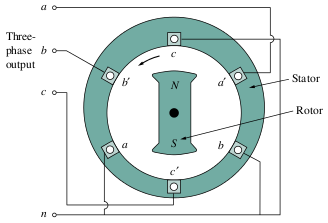
\includegraphics[scale=0.75]{generator.png}
	\caption{Generador Trifásico. (Imagen tomada de \cite{sadiku}, página 479)}
	\label{fig1}
\end{figure}
\noindent
El generador consiste básicamente en un imán rotatorio; llamado \textbf{rotor}; rodeado por una bobina estacionaria; llamada \textbf{estator}. Tres arrollamientos o bobinas separadas con los terminales $a - a'$, $b - b'$ y $c - c'$ aproximadamente en $120^{\circ}$ al rededor de todo el estator. Las tensiones inducidas en las bobinas son iguales en magnitud, pero desfasadas en $120^{\circ}$, como el la Fig. \ref{fig2}
\begin{figure}[H]
	\centering
		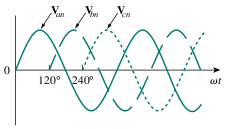
\includegraphics[scale=0.9]{outgenerator.png}
	\caption{Salida del generador de la Fig. \ref{fig1}. (Imagen tomada de \cite{sadiku}, página 479)}
	\label{fig2}
\end{figure}
\noindent
Las fuentes de tensión pueden ser conectados en estrella (Y), como se muestra en la Fig. \ref{figa} o en triángulo ($\Delta$) como en la Fig. \ref{figb}.
\begin{figure}[H]
  \centering
    \subfigure[Conexión en estrella (Y)]{\label{figa}
      \fbox{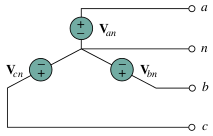
\includegraphics[scale=0.7]{estrella.png}}}
  \hspace{2cm}
    \subfigure[Conexión en triangulo ($\Delta$)]{\label{figb}
      \fbox{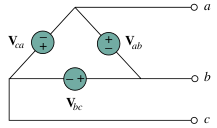
\includegraphics[scale=0.7]{delta.png}}}
  \caption{Fuentes de Voltaje Trifásica. (Imágenes tomadas de \cite{sadiku}, Página 480)}
    \label{fig3}
\end{figure}
\noindent
Para que el sistema se encuentre balanceado es necesario que se cumpla la ecu. \ref{ecu1} y la ecu. \ref{ecu2}.
\begin{equation}
 {V_{an}} + {V_{bn}} + {V_{cn}} = 0
\label{ecu1}
\end{equation}
\begin{equation}
 \left| {V_{an}} \right| = \left| {{V_{bn}}} \right| = \left| {{V_{cn}}} \right|
\label{ecu2}
\end{equation}
\noindent
Existen 2 tipos de secuencia para los sistemas balanceados, si es de \textbf{secuencia positiva} se expresa de la siguiente manera
\begin{equation}
 \begin{array}{l}
 {V_{an}} = {V_p}\angle 0^\circ  \\ 
 {V_{bn}} = {V_p}\angle  - 120^\circ  \\ 
 {V_{cn}} = {V_p}\angle  - 240^\circ  = {V_p}\angle 120^\circ  \\ 
 \end{array}
\label{ecu3}
\end{equation}
\begin{figure}[H]
	\centering
		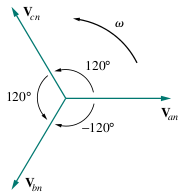
\includegraphics[scale=0.75]{positiva.png}
	\caption{Secuencia Positiva. (Imagen tomada de \cite{sadiku}, página 480)}
	\label{fig4}
\end{figure}
\noindent
si es de \textbf{secuencia negativa} se expresa de la siguiente manera
\begin{equation}
 \begin{array}{l}
 {V_{an}} = {V_p}\angle 0^\circ  \\ 
 {V_{cn}} = {V_p}\angle  - 120^\circ  \\ 
 {V_{bn}} = {V_p}\angle  - 240^\circ  = {V_p}\angle 120^\circ  \\ 
 \end{array}
\label{ecu4}
\end{equation}
\begin{figure}[H]
	\centering
		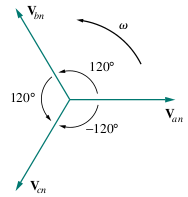
\includegraphics[scale=0.75]{negativa.png}
	\caption{Secuencia Negativa. (Imagen tomada de \cite{sadiku}, página 480)}
	\label{fig5}
\end{figure}
\noindent
Al igual que las conexiones del generador, una carga trifásica puede ser conectada en estrella o delta,de acuerdo a la aplicación final. La Fig. \ref{fig6a} muestra una carga conectada en estrella, y la Fig. \ref{fig6b} muestra una carga conectada en delta.
\begin{figure}[H]
  \centering
    \subfigure[Conexión de cargas en estrella (Y)]{\label{fig6a}
      \fbox{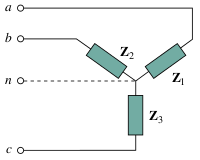
\includegraphics[scale=0.6]{loadestrella.png}}}
  \hspace{2cm}
    \subfigure[Conexión de cargas en triangulo ($\Delta$)]{\label{fig6b}
      \fbox{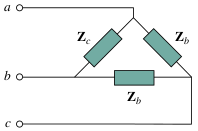
\includegraphics[scale=0.63]{loaddelta.png}}}
  \caption{Fuentes de Voltaje Trifásica. (Imágenes tomadas de \cite{sadiku}, Página 481)}
    \label{fig6}
\end{figure}
\noindent
Una \textbf{carga balanceada} es aquella en la que las impedancias de fase son iguales en magnitud y en fase.\\
Para una carga balanceada conectada en Y,
\begin{equation}
 Z_1=Z_2=Z_3=Z_Y
\label{ecu5}
\end{equation}
\noindent
donde $Z_Y$ es la impedancia de carga por fase. Para una carga balanceada conectada en $\Delta$,
\begin{equation}
 Z_a=Z_b=Z_c=Z_{\Delta}
\label{ecu6}
\end{equation}
\noindent
donde $Z_{\Delta}$ es la impedancia de carga por fase.
\begin{equation}
 Z_{\Delta} =3 Z_{Y}\ \ \ \ \ or \ \ \ \ \ Z_{Y} =\frac{1}{3} Z_{\Delta}
\label{ecu7}
\end{equation}
\noindent
Una carga conectada en estrella se puede transformar en una carga conectada en delta, o viceversa, usando la ecu. (\ref{ecu7}).

\subsection{Conexión Balanceada Y-Y}
Un sistema Y-Y balanceado es un sistema de tres fases fuentes balanceadas en conexión Y, y una carga balanceada conectada en Y.\\
Un sistema de $4$ hilos en conexión Y-Y Fig. \ref{fig7}
\begin{figure}[H]
	\centering
		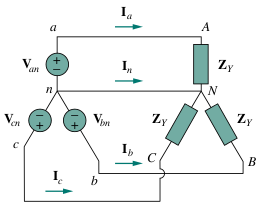
\includegraphics[scale=0.75]{yybalanceado.png}
	\caption{Conexión Y-Y Balanceada. (Imagen tomada de \cite{sadiku}, página 483)}
	\label{fig7}
\end{figure}
\noindent
donde $Z_Y$ es la impedancia de carga de cada fase. Asumiendo una secuencia positiva los voltajes de fase son
\begin{equation}
 V_{an} = V_{p} \angle 0 ^ {\circ}\ \ \ V_{ab} = V_{p} \angle -120 ^ {\circ}\ \ \ V_{cn} = V_{p} \angle 120 ^ {\circ}
\label{ecu8}
\end{equation}
\noindent
Los voltajes de línea $V_{ab}$, $V_{bc}$ y $V_{ca}$, están relacionados con los voltajes de fase.
\begin{equation}
 V_{ab} = V_{an} - V_{bn} = V_{p} \angle 0^{\circ} -V_{p} \angle -120^{\circ} = \sqrt{3}V_{p} \angle\ \ 30^{\circ}
\label{ecu9}
\end{equation}
\noindent
De manera similar se obtiene
\begin{equation}
 V_{bc} = V_{bn} - V_{cn} = \sqrt{3}V_{p} \angle\ \ -90^{\circ}
\label{ecu10}
\end{equation}
\begin{equation}
 V_{ca} = V_{cn} - V_{an} = \sqrt{3}V_{p} \angle\ \ -210^{\circ}
\label{ecu11}
\end{equation}
\noindent
Por lo tanto, la magnitud de los voltajes de línea $V_L$ es $\sqrt{3}$ veces la magnitud del voltaje de fase $V_p$, ​​o
\begin{equation}
 V_L = \sqrt{3} V_{P}
\label{ecu12}
\end{equation}
\noindent
donde
\begin{equation}
 {V_p} = \left| {{V_{an}}} \right| = \left| {{V_{bn}}} \right| = \left| {{V_{cn}}} \right|
\label{ecu13}
\end{equation}
\noindent
y
\begin{equation}
 {V_L} = \left| {{V_{ab}}} \right| = \left| {{V_{bc}}} \right| = \left| {{V_{ca}}} \right|
\label{ecu14}
\end{equation}
\begin{figure}[H]
	\centering
		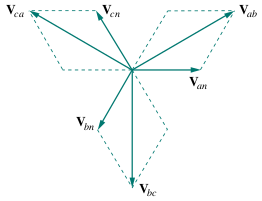
\includegraphics[scale=0.75]{diagramafase.png}
	\caption{Diagrama de fase. Relación entre voltajes de línea y voltajes de fase. (Imagen tomada de \cite{sadiku}, página 484)}
	\label{fig8}
\end{figure}
\noindent
Si se le aplica ley de voltajes de Kirchhoff a la Fig. \ref{fig7} se obtienen las siguientes corrientes de línea
\begin{equation}
 I_a = \frac{V_{an}}{Z_Y}
\label{ecu15}
\end{equation}
\begin{equation}
 I_b= \frac{V_{bn}}{Z_Y} = \frac{V_{an}\angle -120 ^{\circ}}{Z_Y}= I_a \angle -120 ^{\circ}
\label{16}
\end{equation}
\begin{equation}
 I_c= \frac{V_{cn}}{Z_Y} = \frac{V_{an}\angle 120 ^{\circ}}{Z_Y}= I_a \angle 120 ^{\circ}
\label{17}
\end{equation}
\noindent
Se puede deducir fácilmente que las corrientes de línea son iguales a cero,
\begin{equation}
 I_a + I_b + I_c = 0
\label{ecu18}
\end{equation}
\noindent
de modo que
\begin{equation}
 {I_n} =  - \left( {{I_a} + {I_b} + {I_c}} \right) = 0
\label{ecu19}
\end{equation}
\noindent
o
\begin{equation}
 V_{nN}= Z_n I_n = 0
\label{ecu20}
\end{equation}
\noindent
es decir, la tensión en el cable neutro es igual a cero, dicha línea puede ser removida y no afectara el sistema. Los sistemas de potencia diseñados de esta manera se encuentran bien fundamentados en todos los puntos críticos para garantizar la seguridad.\\
Mientras que la formación actual es la corriente en cada línea, la corriente de fase es la corriente en cada fase de la fuente o la carga. En el sistema de Y-Y, la corriente de línea es como la corriente de fase.

\subsection{Conexión Balanceada Y-$\Delta$}
\noindent
Un sistema balanceado Y-$\Delta$ es como la Fig. \ref{fig9}, conectando fuentes balanceadas en Y y cargas balanceadas en $\Delta$.
\begin{figure}[H]
	\centering
		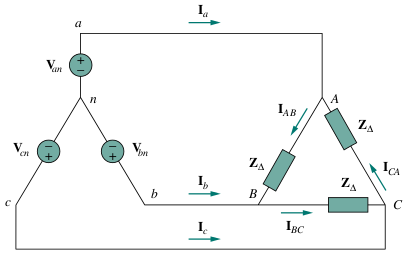
\includegraphics[scale=0.6]{ydelta.png}
	\caption{Conexión Balanceada Y-$\Delta$. (Imagen tomada de \cite{sadiku}, página 486)}
	\label{fig9}
\end{figure}
\noindent
Asumiendo una secuencia positiva como en la ecu. (\ref{ecu3}), entonces los voltajes de línea son:
\begin{equation}
 V_{ab} = \sqrt{3} V_p \angle\ 30 ^{\circ} = V_{AB}
\label{ecu21}
\end{equation}
\begin{equation}
 V_{bc} = \sqrt{3} V_p \angle\ -90 ^{\circ} = V_{BC}
\label{ecu22}
\end{equation}
\begin{equation}
 V_{ca} = \sqrt{3} V_p \angle\ 150 ^{\circ} = V_{CA}
\label{ecu23}
\end{equation}
\noindent
dado que las tensiones de línea son iguales a las tensiones a través de las impedancias de carga en esta configuración del sistema. A partir de estas tensiones, se obtienen las corrientes de fase:
\begin{equation}
 I_{AB} = \frac{V_{AB}}{Z_{\Delta}}, \ \ \ I_{BC} = \frac{V_{BC}}{Z_{\Delta}}, \ \ \ I_{CA} = \frac{V_{CA}}{Z_{\Delta}}
\label{ecu24}
\end{equation}
\noindent
Para hallar las corrientes de línea se utiliza la ley de corrientes de Kirchhoff a los nodos $A$, $B$ y $C$
\begin{equation}
 I_a = I_{AB} - I_{CA} \ \ \ I_b = I_{BC} - I_{AB} \ \ \ I_c = I_{CA} - I_{BC}
\label{ecu25}
\end{equation}
\noindent
Como $I_{CA} = I_{AB} \angle\ 120^\circ$
\begin{equation}
 I_a =I_{AB} - I_{CA} = I_{AB}(1 - 1\angle\ 120^\circ) = I_{AB} \sqrt{3}\angle\ -30^\circ
\label{ecu26}
\end{equation}
\noindent
Por lo tanto, la magnitud de los corrientes de línea $I_L$ es $\sqrt{3}$ veces la magnitud de la corriente de fase $I_p$, ​​o
\begin{equation}
 I_L = \sqrt{3} I_{P}
\label{ecu27}
\end{equation}
\noindent
Es decir, las magnitudes de las corrientes de linea son iguales entre ellas y las magnitudes de las corrientes de fase también lo son.
\begin{figure}[H]
	\centering
		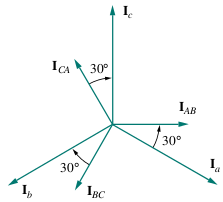
\includegraphics[scale=0.7]{diagramacorrientes.png}
	\caption{Diagrama de fase. Relación entre las corrientes de línea y de fase. (Imagen tomada de \cite{sadiku}, página 487)}
	\label{fig10}
\end{figure}

\subsection{Conexión Balanceada $\Delta$-$\Delta$}
\noindent
Un sistema balanceado $\Delta$-$\Delta$ es un sistema en el que tanto las fuentes como la cargas se encuentran balanceadas y conectadas en $\Delta$ Fig. \ref{fig11}.
\begin{figure}[H]
	\centering
		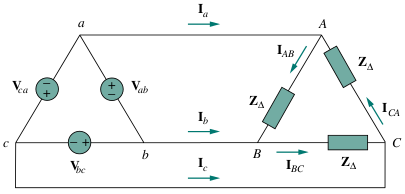
\includegraphics[scale=0.6]{deltadelta.png}
	\caption{Conexión $\Delta$-$\Delta$ Balanceada. (Imagen tomada de \cite{sadiku}, página 489)}
	\label{fig11}
\end{figure}
\noindent
Asumiendo una secuencia positiva como para los voltajes de fase para la conexión $\Delta$ de las fuentes
\begin{equation}
 V_{ab} = V_p \angle\ 0^\circ,\ \ \ V_{bc} = V_p \angle -120^\circ,\ \ \ V_{ca} = V_p \angle\ 120^\circ
\label{ecu28}
\end{equation}
\noindent
Los voltajes de línea son como los voltajes de fase. Para la Fig. \ref{fig11} los voltajes de fase de la conexión $\Delta$ de las fuentes es el mismo voltaje sobre la impedancia
\begin{equation}
 V_{ab} = V_{AB}, \ \ \ \ V_{bc} = V_{BC}, \ \ \ \ V_{ca} = V_{CA}
\label{ecu29}
\end{equation}
\noindent
Entonces la corriente de fase
\begin{equation}
 I_{AB} = \frac{V_{AB}}{Z_{\Delta}} = \frac{V_{ab}}{Z_{\Delta}}
\label{ecu30}
\end{equation}
\begin{equation}
 I_{BC} = \frac{V_{BC}}{Z_{\Delta}} = \frac{V_{bc}}{Z_{\Delta}}
\label{ecu31}
\end{equation}
\begin{equation}
 I_{CA} = \frac{V_{CA}}{Z_{\Delta}} = \frac{V_{ca}}{Z_{\Delta}}
\label{ecu32}
\end{equation}
\noindent
Para obtener las corrientes de linea se debe aplicar Ley de corrientes de Kirchhoff a los nodos $A$, $B$ y $C$
\begin{equation}
 I_a = I_{AB} - I_{CA} \ \ \ I_b = I_{BC} - I_{AB} \ \ \ I_c = I_{CA} - I_{BC}
\label{ecu33}
\end{equation}
\noindent
Como se ha mencionado anteriormente la corriente de línea es la corriente de fase por $30 ^\circ$, la magnitud de la corriente de línea $V_L$ es $\sqrt{3}$ veces la magnitud del voltaje de fase $I_p$,
\begin{equation}
 I_L = \sqrt{3}\ I_p
\label{ecu34}
\end{equation}

\subsection{Conexión Balanceada $\Delta$-Y}
\noindent
Un sistema balanceado $\Delta$-Y consiste en una conexión de fuentes balanceadas en $\Delta$, conectadas a una carga balanceada en Y, Fig. \ref{fig12}
\begin{figure}[H]
	\centering
		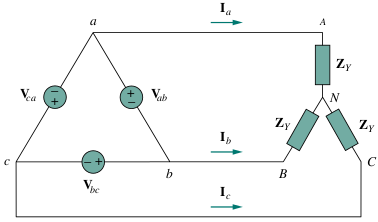
\includegraphics[scale=0.65]{deltay.png}
	\caption{Conexión $\Delta$-Y Balanceada. (Imagen tomada de \cite{sadiku}, página 491)}
	\label{fig12}
\end{figure}
\noindent
Consideremos una secuencia positiva como la ecu. (\ref{ecu28}). Cuando se aplica Ley de voltajes de Kirchhoff a la Fig. \ref{fig12}
\begin{equation}
 -V_{ab} + Z_Y I_a - Z_Y I_b = 0
\label{ecu35}
\end{equation}
\begin{equation}
 Z_Y ( I_a - I_b ) = V_{ab} = V_p \angle\ 0 ^ \circ
\label{ecu36}
\end{equation}
\noindent
entonces
\begin{equation}
 I_a - I_b = \frac{V_p \angle \ 0 ^\circ }{Z_Y}
\label{ecu37}
\end{equation}
\noindent
Pero $I_b$ atrasa a $I_a$ por $120 ^ \circ$, asumiendo una secuencia positiva $I_b = I_a \angle -120 ^ \circ$, entonces
\begin{equation}
 I_a - I_b = I_a(1 - 1 \angle -120 ) = I_a \sqrt{3} \angle\ 30 ^ \circ
\label{ecu38}
\end{equation}
\noindent
Sustituyendo la ecu. (\ref{ecu38}) en la ecu. (\ref{ecu37})
\begin{equation}
 I_a = \frac{V_p / \sqrt{3}\angle -30 ^ \circ}{Z_Y}
\label{ecu39}
\end{equation}
\noindent
Las corrientes de línea $I_b$ y $I_c$ usando la secuencia positiva se obtiene $I_b = I_a \angle -120 ^ \circ$, $I_c = I_a \angle\ 120 ^ \circ$

\subsection{Potencia en sistemas balanceados}
\noindent
Para analizar potencia instantánea absorbida por la carga es necesario analizarlo en el dominio del tiempo. Para una conexión en Y de la carga el voltaje de fase es
\begin{equation}
 v_{AN} = \sqrt{2}V_p cos \omega t
\label{ecu40}
\end{equation}
\begin{equation}
 v_{BN} = \sqrt{2}V_p cos( \omega t -120 ^\circ)
\label{ecu41}
\end{equation}
\begin{equation}
 v_{CN} = \sqrt{2}V_p cos( \omega t +120 ^\circ)
\label{ecu42}
\end{equation}
\noindent
donde $\sqrt{2}$ es necesario porque $V_p$ se ha definido como voltaje $RMS$ para el voltaje de fase. Si $Z_Y = Z \angle \theta$ la corriente de fase atrasa el correspondiente voltaje de fase por $\theta$
\begin{equation}
 i_a= \sqrt{2} I_p cos (\omega t - \theta)
\label{ecu43}
\end{equation}
\begin{equation}
 i_b= \sqrt{2} I_p cos (\omega t - \theta - 120 ^ \circ)
\label{ecu44}
\end{equation}
\begin{equation}
 i_c= \sqrt{2} I_p cos (\omega t - \theta + 120 ^ \circ)
\label{ecu45}
\end{equation}
\noindent
donde $I_p$ es el valor $RMS$ del valor de la corriente de fase. La potencia total instantánea en la carga es la suministrada por la potencia instantánea en las $3$ fases
\begin{equation}
 p = p _a + p_b + p_c = v_{AN} i_a +v_{BN} i_b + v_{cN} i_c
\label{ecu46}
\end{equation}
\noindent
al sustituir los voltajes en la ecu. (\ref{ecu46}) y aplicando la identidad trigonométrica, se obtiene
\begin{equation}
 p = 3 V_p I_p cos \theta
\label{ecu47}
\end{equation}
\noindent
Los resultados son los mismos para las diferentes combinaciones de sistemas trifásicos. La medida de la potencia instantánea total por fase $P_p$ para la cualquier combinación de la carga es $p/3$, o
\begin{equation}
 P_p = V_p I_p cos \theta
\label{ecu48}
\end{equation}
\noindent
por consiguiente la potencia reactiva por fase será
\begin{equation}
 Q_p = V_p I_p sin \theta
\label{ecu49}
\end{equation}
\noindent
la potencia aparente por fase será
\begin{equation}
 S_p = V_p I_p
\label{ecu50}
\end{equation}
\noindent
la potencia compleja por fase será
\begin{equation}
 S_p = P_p + iQ_p = V_p I^{*}_p
\label{ecu51}
\end{equation}
\noindent
donde $V_p$ e $I_p$ son los voltajes y corrientes de fase, con magnitudes $V_p$ e $I_p$, respectivamente. la medida total de la potencia es la suma de las potencias de cada fase
\begin{equation}
 P = P_a + P_b + P_c = 3P_p = 3 V_p I_p cos \theta = \sqrt{3} V_L I_L cos \theta
\label{ecu52}
\end{equation}
\noindent
de igual manera la potencia total reactiva será
\begin{equation}
 Q = 3 V_p I_p sin \theta = 3 Q_p = \sqrt{3} V_L I_L sin \theta
\label{ecu53}
\end{equation}
\noindent
la potencia compleja total será
\begin{equation}
 S = 3 S_p = 3 V_p I^{*}_p = 3 I ^ {2} _p Z_p = \frac{3 V^{2}_p}{Z^{*}_p}
\label{ecu54}
\end{equation}
\noindent
donde $Z_p = Z_p \angle \theta$ es la impedancia total por fase, la ecu. (\ref{ecu54}) se puede escribir como
\begin{equation}
 S = P + iQ = \sqrt{3} V_L I_L \angle \theta
\label{ecu55}
\end{equation}

\section{Hipótesis}
\noindent
Al medir la potencia con el método de los dos watimetros la suma de la potencia activa registrada por cada uno será la potencia trifásica total que consume la carga.\\
Los voltajes de línea serán mayores en una magnitud de $\sqrt{3}$ a los voltajes de fase en una conexión estrella-estrella (Y-Y).\\
Las corrientes de línea serán mayores en una magnitud de $\sqrt{3}$ a las corrientes de fase en una conexión estrella-delta (Y-$\Delta$).

\section{Materiales}
\begin{itemize}
 \item Bombillos
 \item Borneras
 \item Diodos
 \item Multímetro
 \item Pinza o tranformador de corriente
 \item Rosetas
 \item Vatímetros
\end{itemize}

\section{Análisis y Resultados Teórico}
\noindent
Para esta práctica se implementaran tres circuitos trifásicos con fuentes balanceadas, a continuación se muestran los montajes de estos.

\subsection{Circuito $Y-Y$}
\noindent
Para esta parte de la práctica se implementa el siguiente circuito trifásico $Y-Y$ con cargas balanceadas para el cual se hace el análisis correspondiente.
\begin{figure}[H]
	\centering
		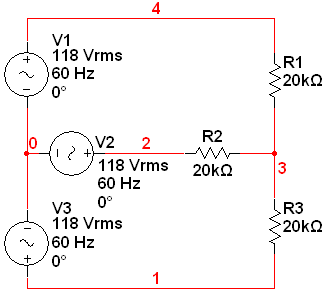
\includegraphics[scale=0.7]{circYY.PNG}
	\caption{Circuito Balanceado $Y-Y$}
	\label{fig13}
\end{figure}
\noindent
Al tener el circuito con carga balanceada se puede decir que la tensión el Nodo $3$ es $0\ V$, lo cual facilita el análisis ya que en cada resistencia $Z_Y$ cae  una tensión de $120\ V_{RMS}$.
\begin{equation}
 {I_a} =\frac {V_{an}}{Z_Y} =\frac {120 \angle 0^\circ V}{ 20 \angle 0^\circ\ K \Omega}= 6\angle 0°\ mA
\label{ecu56}
\end{equation}
\noindent
De igual forma se obtiene  $I_b= 6\angle -120^\circ\ mA$ y $I_c= 6\angle 120^\circ \ mA$.
\begin{equation}
 P = 3  V_f  I_L  cos \theta = 3(120 V)(6 mA)Cos 0^\circ = 2.16\ Watts
\label{ecu57}
\end{equation}

\subsection{Circuito $Y-\Delta$}
\noindent
A continuación se muestra el circuito Y-$\Delta$ con carga balanceada, para este circuito se hace el análisis pertinente.
\begin{figure}[H]
	\centering
		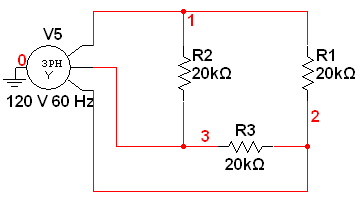
\includegraphics[scale=0.7]{circYD.PNG}
	\caption{Circuito Balanceado $Y-\Delta$}
	\label{fig14}
\end{figure}
\noindent
Nuevamente se tiene un circuito balanceado se facilita el análisis teniendo.
\begin{equation}
 V_L = \sqrt(3)120 \angle \emptyset V =V_{Z\Delta}
 \label{ecu58}
\end{equation}
\noindent
Para esta tensión de línea $V_L$ el ángulo $\emptyset$ cumple el sistema balanceado.
\begin{equation}
 I_L =\frac{V_L}{Z_{\Delta}}=\frac{\sqrt(3)120 \angle \emptyset V}{20 \angle 0^\circ\ K \Omega}=10.392\angle \emptyset mA
 \label{ecu59}
\end{equation}
\noindent
Las corrientes de línea $I_L$, de igual forma tienen ángulos $\emptyset$ balanceados.
\begin{equation}
 P = \sqrt(3)  V_L  I_L  cos \theta
\label{ecu60}
\end{equation}
\begin{equation}
 P =\sqrt(3)(\sqrt(3)120 V)(10.392 mA)cos 0^\circ = 3.741\ Watts
\label{ecu61}
\end{equation}

\subsection{Rectificación de media Onda}
\noindent
En la práctica se diseñara el circuito pertinente para esta parte, con ayuda de la profesora porque no se entendió lo que se quería plantear.

\section{Preguntas}
\begin{enumerate}
 \item ¿Qué relación existe entre voltaje Fase-Fase y fase neutro?\\
En el caso de una fuente trifásica balanceada la magnitud del voltaje Fase-Fase es mayor en un termino de $\sqrt{3}$ a la magnitud del voltaje fase-neutro, además existe una diferencia entre al ángulo de fase de $30^\circ$ dependiendo si la fuente esta en secuencia positiva o negativa, así en secuencia positiva el ángulo del voltaje de Fase-Fase esta en adelanto de $30^\circ$ respecto al ángulo de voltaje de fase-neutro, y en secuencia negativa el ángulo del voltaje de Fase-Fase esta en atraso de $30^\circ$ respecto al ángulo de voltaje de fase-neutro
 \item ¿Que son, como se usan y que limitaciones tienen los Diodos de potencia?\\
Es un dispositivo unidireccional que permite el paso de corriente en un solo sentido; cuando el diodo de potencia se encuentra en estado de conducción debe ser capaz de soportar un alta corriente con una pequeña caída de tensión. En sentido inverso soportan una fuerte tensión negativa de ánodo con una pequeña corriente inversa.
\begin{figure}[H]
	\centering
		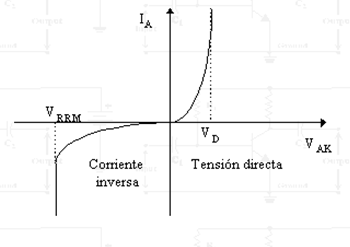
\includegraphics[scale=0.7]{diodo.png}
	\caption{Gráfica de funcionamiento del diodo}
	\label{fig20}
\end{figure}

 \item ¿Qué es y como se puede medir la potencia activa, reactiva y aparente?\\
La potencia aparente de un circuito eléctrico de corriente alterna magnitud se identifica con la letra S y es la suma vectorial de la potencia que disipa dicho circuito y se transforma en calor o trabajo, que es conocida como potencia real o activa , que se designa con la letra P y se mide en vatios ($W$) y la potencia utilizada para la formación de los campos eléctrico y magnético de sus componentes, que se denomina como potencia reactiva, se designa con la letra $Q$ y se mide en volt-amperios reactivos ($VAR$). La relación entre la magnitud de  potencia aparente, la activa y la reactiva es:
\begin{equation}
 S^2=P^2_{A}+Q^2_{R}
\label{ecu70}
\end{equation}
\noindent
Y vectorialmente:
\begin{equation}
 S=P_A cos\theta+iQ_R sin\theta
\label{ecu71}
\end{equation}
\noindent
La potencia activa se puede medir utilizando un watimetro, ya que es un dispositivo que mide simultáneamente la corriente y el voltaje. En un sistema trifásico se utiliza la conexión de dos watimetros donde la suma de sus potencias medidas es la potencia total del circuito.\\
Utilizando el método de los dos watimetros es posible establecer el ángulo entre el voltaje y la corriente:
\begin{equation}
 \theta  = {\rm{arctan}}\left( {\frac{{\sqrt 3 ({W_2} - {W_1})}}{{{W_1} + {W_2}}}} \right)
\label{ecu72}
\end{equation}
\noindent
Una vez conocido el ángulo podemos determinar la magnitud de la potencia aparente $S$:
\begin{equation}
 S=\frac{P_A}{cos \theta}
\label{ecu73}
\end{equation}
La magnitud de la potencia reactiva será:
\begin{equation}
 Q_R=S sen \theta
\label{ecu74}
\end{equation}

 \item ¿Cómo se mide la energía consumida por el sistema?\\
La potencia es la velocidad con la que se consume la energía, entonces para determinar cuanta energía consume el sistema debemos considerar un intervalo de tiempo y el producto de la potencia medida por el tiempo será la energía.
\end{enumerate}

\bibliographystyle{ieeetran}
\begin{thebibliography}{99}
\bibitem{sadiku} Alexander, Charles K. \&  Sadiku, Matthew N.O.
{\em ```Fundamentals of Electric Circuits"'}.
McGRAW-HILL, ISE Editions, 1999.

\bibitem{dorf} Dorf  \& Svoboda.
{\em ```Circuitos Eléctricos"'}.
Alfaomega, Sexta Edición, 2006.

\bibitem{hayt} Hayt, William H. Jr., Kemmerly, Jack E. \& Durbin, Steven M.
{\em ```Análisis de circuitos en ingeniería"'}.
McGRAW-HILL, Séptima Edición, 2007.

\bibitem{nahvi} Nahvi, Mahmood \& Edminister, Joseph A.
{\em ```Theory and Problems of Electric Circuits"'}.
McGRAW-HILL, Fourth Edition, 2003.

\end{thebibliography}
\end{document}